\secput{appendix}{Appendix}

\subsecput{apdx-meta-intro}{Meta-algorithm for $2$-D grids} 

From the results in \cite{Yao82, Yao85, Seidel06}, we can establish
following recurrence for space and time bound of $1$-D
preprocessing algorithm.

\begin{eqnarray}
\mathcal{S}_{1, 0} (n) & = & n \log n \hfil \mbox{// initial algo} \\
\mathcal{S}_{1, 1} (n) & = & \Theta(n) + \mathcal{S}_{1, 0}(n/\log n) + n/\log n \cdot \mathcal{S}_{1, 1}(\log n) \hfil \mbox{// use $\mathcal{S}_{1, 0}$ inter-block query}\\
\ldots & = & \ldots \\
\mathcal{S}_{1, k} (n) & = & \Theta(n) + \mathcal{S}_{1, k-1}(n / f(n)) + n/f(n) \cdot \mathcal{S}_{1, k}(f(n)) \hfil \mbox{// Suppose the complexity of $\mathcal{S}_{1, k-1}(n) = n f(n)$} \\ 
\mathcal{S}_{1, \alpha(n)} (n) & = & \Theta(n \alpha (n)) \\ 
\label{eq:meta-1D-S1}
\end{eqnarray}

For the notation $\mathcal{S}_{d, k}$, $\mathcal{S}$ stands for the
space and time bound, the first subscript stands for dimensionality,
the second is the recursion level. Similarly, we have a recurrence
for query overhead, where $\mathcal{Q}$ stands for the query overhead,
the semantics of subscript is the same as in $\mathcal{S}_{d, k}$:

\begin{eqnarray}
\mathcal{Q}_{1, 0} & = & 1 \hfil \mbox{// initial algo}\\
\mathcal{Q}_{1, 1} & = & 2 + \mathcal{Q}_{1, 0} \hfil \mbox{// any query can be decomposed into at most one inter-block query and one suffix/prefix} \\
\ldots & = & \ldots \\
\mathcal{Q}_{1, k} & = & 2 + \mathcal{Q}_{1, k-1} \\
\mathcal{Q}_{1, \alpha(n)} & = & \Theta(\alpha(n))
\label{eq:meta-1D-Q1}
\end{eqnarray}

To extend the same kind of recurrence to multi-dimensional grids,
we start from how to use meta-algorithm to process a $2$-D
grid and iteratively apply to itself to achieve alpha bound. 
First, we need an initial algorithm to kick
off. The initial algorithm doesn't need to be very smart, it just needs
to work. Our meta-algorithm will later transform it through a series
of recursion levels and improves the asymptotic bound to eventually hit
the alpha bound.

\subsubsecput{apdx-init-2D}{Initial algorithm for $2$D grids}

\begin{figure*}[!ht]
\centering
\subfigure[Initial algorithm for $2$D orthogonal range queries]{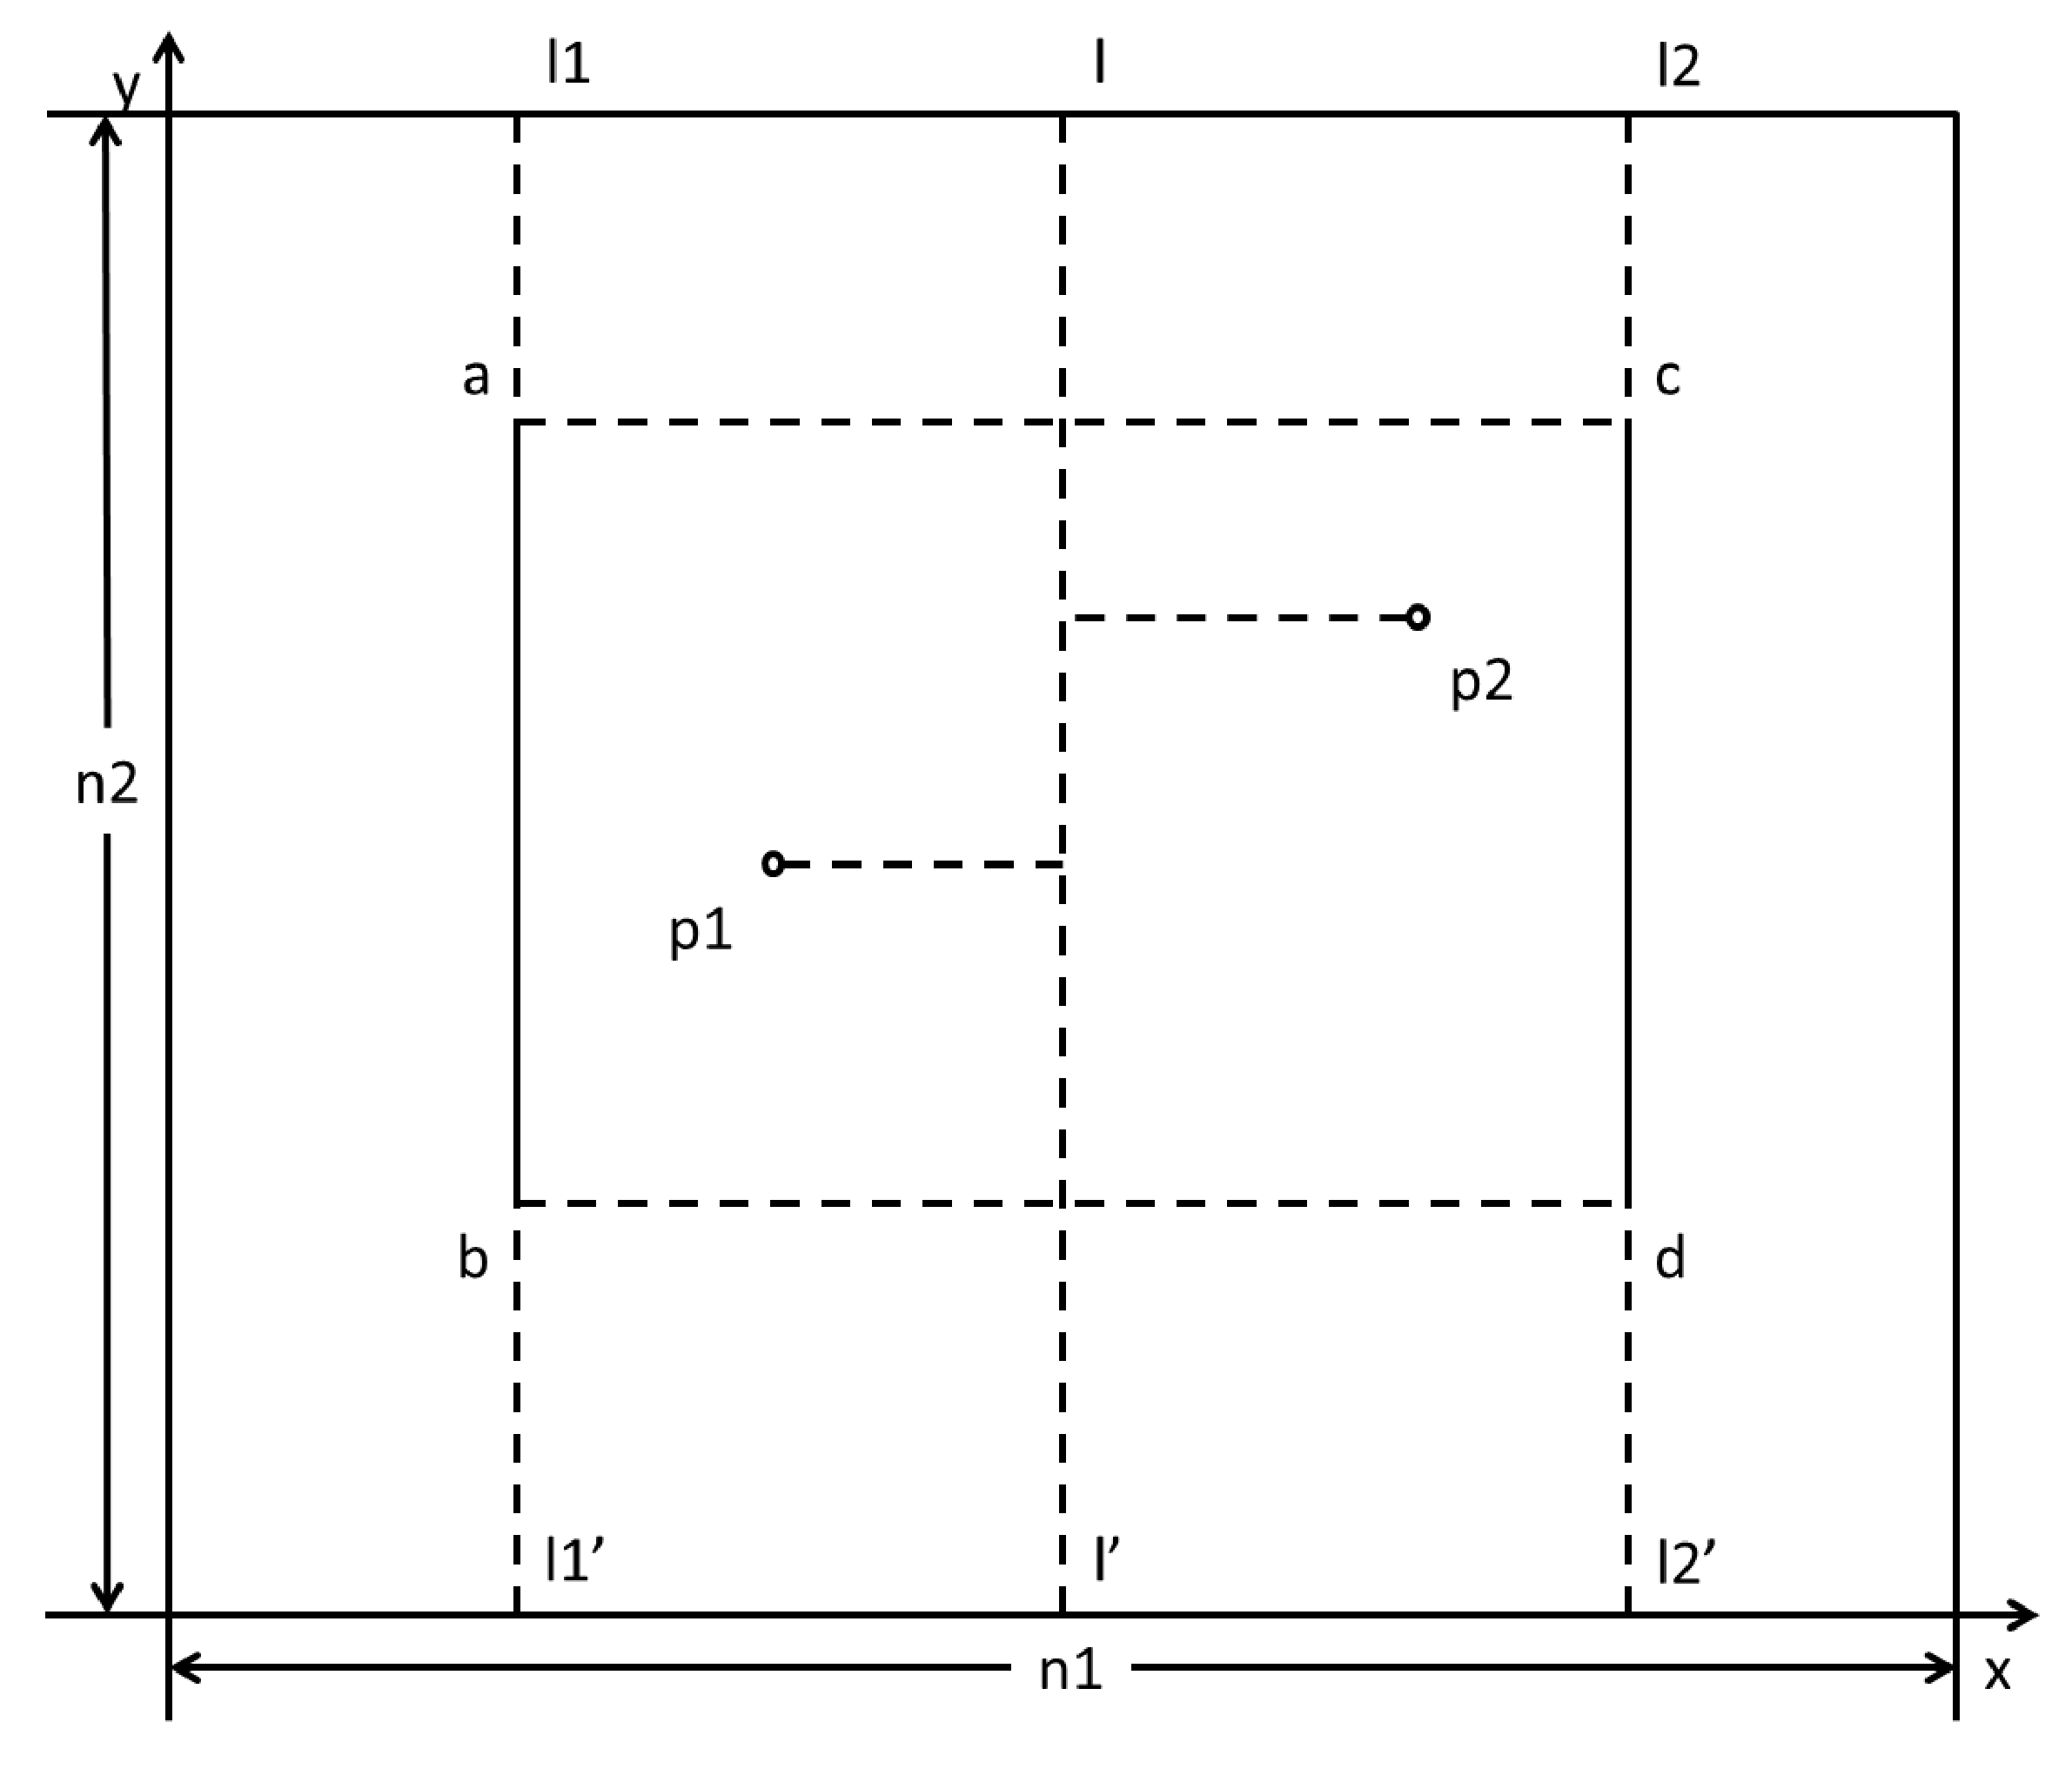
\includegraphics[clip,width=3in]{figures/init_2D.eps}
\label{fig:init-2D}}
\hfill
%\hspace{0.01cm}
\subfigure[Meta-algorithm for $2$D orthogonal range queries]{\includegraphics[clip,width=3in]{figures/meta_2D.eps}
\label{fig:meta-2D}
}
\caption{Initial and meta-algorithm for $2$-D orthogonal range queries}
\label{fig:twod}
\end{figure*}

As shown in \figref{init-2D}, the initial algorithm is a direct extension
of A. Yao's initial algorithm \cite{Yao82} to $2$-D grids. The algorithm
is diagrammed in \figref{init-2D}. The description is as follows and uses
the notation in \figref{init-2D}, the pseudo-code is in \figref{init-2D-algo}

\begin{enumerate}
\item Select a longer dimension, without loss of generality, let's
  suppose it's dimension $\id{x}$.
\item Partition dimension $\id{x}$ by a center line $\overline{\id{ll'}}$
  into evenly two parts. Then all points in the grid resides
  either on the left (e.g.  $\id{p_1}$) of the center line or right
  (e.g. $\id{p_2}$). For all the points, reducing (by applying the $\oplus$
  operator) the data from center line to itself by dynamic programming.
  We call the reduced data prefix or suffix value from the center line.
\item After data reduction on both prefix and suffix values, applying Yao's
  initial $1$-D preprocessing algorithm \cite{Yao82, ChazelleRo91},
  which has complexity $O(n \log (n))$ on all lines along vertical
  dimension $\id{y}$.
\item Now we have the observation that all $2$-D orthogonal range query
  that spans across the center line $\overline{\id{ll'}}$ can be
  answered by conducting two $1$-D queries on both left-hand side
  and right-hand side of the center line. E.g. To query the rectangle
  $\Box\id{abdc}$ in \figref{init-2D}, we perform one $1$-D query
  on line $\overline{\id{l_1l_1'}}$ and another $1$-D query on line
  $\overline{\id{l_2l_2'}}$. Combining these two results by $\oplus$
  operator, we get the final query result of the orthogonal range query.
\item Recursively applying the above procedure to the left and right
  sub-grids of line $\overline{\id{ll'}}$.
\end{enumerate}

\begin{theorem}
The preprocessing of Algoritm~\figref{init-2D} has complexity of
$\mathcal{S}_{2, 0}(n_1, n_2) = \Theta(n_1 \cdot n_2 \cdot \log (n_1)
\cdot \log(n_2))$ in both time and space.
\label{thm:init-2D-pp}
\end{theorem}

\begin{IEEEproof}
Apparently, at each level of recursion, it requires at least $n_1
n_2$ space and time to hold prefix and suffix grids.

For each vertical lines, such as $\overline{\id{l_1l_1'}}$ and
$\overline{\id{l_2l_2'}}$, we apply Yao's initial $1$-D algorithm on it, and
denote it as $\mathcal{S}_{1, 0}(n) = \Theta(n \log n)$. 

Since the partition occurs on dimension $\id{x}$, which will terminate
when the number of vertical lines in the grid less than or equal to $1$,
there are in total $\log n_1$ levels.

Combining all above calculations we have the recurrence:

\begin{eqnarray}
\mathcal{S}_{2, 0} (n_1, n_2) & = & n_1 n_2 + \log n_1 \{ n_1 \cdot \mathcal{S}_{1, 0}(n_2)\} \\
    & = & \Theta(\log n_1 n_1 n_2 \log n_2)
\label{eq:init-2D-S20}
\end{eqnarray}
\end{IEEEproof}

\begin{corollary}
The query overhead of Algorithm~\figref{init-2D} is 
$\mathcal{Q}_{2, 0} = 3-\oplus$
\label{cor:init-2D-query}
\end{corollary}

\begin{IEEEproof}
For the query, we first need to locate which recursion level the query
range resides, which is equivalent to finding the lowest common ancestor
of its range on dimension \id{x}, the overhead of which is not counted
in our simple arithmetic model.
\footnote{In RAM model, by using bit-tricks, finding lowest common
ancestor in a complete binary tree can be accomplished in $O(1)$ time} 

After locating the lowest common ancestor of the query range on dimension
\id{x}, performing two $1$-D queries on left and right-hand side of
the center line of the level, each of which requires 
$\mathcal{Q}_{1, 0} = 1-\oplus$
overhead. In the end, we need to combine both results from two $1$-D
queries into one, which requires another $1-\oplus$ operation. So in
total, we have $\mathcal{Q}_{2, 0} = 2 \mathcal{Q}_{1, 0} + 1 = 3$.
\end{IEEEproof}

\subsubsecput{apdx-meta-2D}{Meta-algorithm for $2$D grids}

The meta-algorithm takes an algorithm as input, such as the initial
algorithm described in ~\figref{init-2D} (\figref{init-2D-algo}),
compress the data alternatively on dimension $\id{x}$ or $\id{y}$ to
eventually hit the $\alpha$ bound. The description follows the notation
in \figref{meta-2D}, the pseudo-code is in \figref{meta-2D-algo}

\begin{enumerate}
\item We start data reduction on a longer dimension,
  without loss of generality, suppose it's dimension $\id{x}$. For
  each line of dimension $\id{y}$, partition it along dimension
  $\id{x}$ into segments of size $\log (\id{x_1} - \id{x_0})$, or
  $\log^* (\id{x_1} - \id{x_0})$, $\log^{**} (\id{x_1} - \id{x_0})$,
  $\ldots$ ($\id{seg\_size}$ in \figref{meta-2D-algo}). The length of
  $\id{seg\_size}$ depends on the complexity of $\id{input\_2D\_algo}$,
  which can be a user's input parameter.
\item For each segment, apply $\oplus$ operator over it and reduce
  all data within the segment into one single value. All such values
  construct a new grid --- $\id{promoted\_grid}$. Applying the
  $\id{input\_2D\_algo}$ to the $\id{promoted\_grid}$.
\item For each vertical line (along dimension $\id{y}$), reduce the
  the data relative to the left and right end of each segment (of
  size $\id{seg\_size}$ to construct the $\id{prefix\_grid}$ and
  $\id{suffix\_grid}$.
\item For each vertical line (e.g. line $\overline{l_1l_1'}$ and
  line $\overline{l_2l_2'}$ in \figref{meta-2D}) in $\id{prefix\_grid}$
  and $\id{suffix\_grid}$, apply the $\id{input\_1D\_algo}$ to it.
  If the $\id{input\_2D\_algo}$ has bound $\Theta(n_1 n_2 f_1(n_1)
  f_2(n_2))$, the corresponding $\id{input\_1D\_algo}$ should be of
  bound $\Theta(n f(n))$, where $f(n) \leq f_1(n)$ and $f(n) \leq f_2(n)$.
\item Recursively apply the meta-algorithm itself on segment blocks
  of size $\id{seg\_size} \times \id{n_2}$. E.g. on colored segment block
  $\Box \id{efgh}$ in \figref{meta-2D}
\item Repeat the above meta-algorithm alternatively on dimension
  $\id{y}$, $\id{x}$.
\end{enumerate}

\begin{theorem}
The preprocessing of Algoritm~\figref{meta-2D} has complexity of 
$\mathcal{S}_{2, \alpha(n_1) \alpha(n_2)} = \Theta(n_1
\cdot n_2 \cdot \alpha (n_1) \cdot \alpha(n_2))$ in both time and space.
\label{thm:meta-2D-pp}
\end{theorem}

\begin{IEEEproof}
\begin{enumerate}
\item In \thmref{init-2D-pp}, we proved that $\mathcal{S}_{2, 0} = 3$.
\item For recursion level $1$: we have $\mathcal{S}_{2, 0}$ as 
  $\id{input\_2D\_algo}$, and $\mathcal{S}_{1, 0}$ as $\id{input\_1D\_algo}$.
  We apply $\id{input\_2D\_algo}$ to $\id{promoted\_grid}$, which is
  of size $n_1/\log n_1 \times n_2$, and apply $\id{input\_1D\_algo}$
  to $\id{prefix\_grid}$ and $\id{suffix\_grid}$, each of which is of
  size $n_1 \times n_2$. So we have the recurrence:
    \begin{eqnarray}
      \mathcal{S}_{2, 1}(n_1, n_2) & = & \mathcal{S}_{2, 0} (n_1/\log n_1,
      n_2) + 2 \times n_1 \times \mathcal{S}_{1, 0} (n_2) 
      \frac{n_1}{\log n_1} \cdot \mathcal{S}_{2, 1}(\log n_1, n_2) \\
          & = & \Theta(n_1 n_2 \log n_2 \log^* n_1)
    \label{eq:meta-2D-S21} 
    \end{eqnarray} 
\item Solution in \eqref{meta-2D-S21} means we now have a $2$-D preprocessing
  algorithm of complexity $O(n_1 n_2 \log^* n_1 \log n_2)$ in both
  space and time. Repeat the same procedure on dimension $\id{y}$, we will 
  have the recurrence:
  \begin{eqnarray}
    \mathcal{S}_{2, 2}(n_1, n_2) & = & \mathcal{S}_{2, 1} (n_1, n_2/\log n_2) 
    + 2 \times n_2 \times \mathcal{S}_{1, 1} (n_1) 
    + \frac{n_2}{\log n_2} \cdot \mathcal{S}_{2, 2}(n_1, \log n_2) \\
        & = & \Theta(n_1 n_2 \log^* n_1 \log^* n_2) 
  \label{eq:meta-2D-S22}
  \end{eqnarray}
\item Repeat above two procedures, more generally, if we assume 
  $\id{input\_2D\_algo}$ has complexity $\Theta(n_1 n_2 f(n_1) f(n_2))$,
  where $f(n) \leq n-2$. We first segment the $2$-D grid along $\id{x}$
  dimension into size of $f(n_1)$ and supply a $1$-D algorithm of
  complexity $\Theta(n f(n))$, we will have the recurrence:
  \begin{eqnarray}
    \mathcal{S}_{2, k}(n_1, n_2) & = & \mathcal{S}_{2, k-1} (n_1/f(n_1), n_2)
    + 2 \times n_1 \times \mathcal{S}_{1, k-1} (n_2)
    + \frac{n_1}{f(n_1)} \cdot \mathcal{S}_{2, k}(f(n_1), n_2) \\
        & = & \Theta(n_1 n_2 f(n_2) f^*(n_1))
  \label{eq:meta-2D-S2k}
  \end{eqnarray}

  In a second step, we supply the $\mathcal{S}_{2, k}$ as 
  $\id{input\_2D\_algo}$ and a $1$-D algorithm of complexity 
  $\mathcal{S}_{1, k} = n f^*(n)$ as $\id{input\_1D\_algo}$.

  \begin{eqnarray}
    \mathcal{S}_{2, k+1}(n_1, n_2) & = & \mathcal{S}_{2, k} (n_1, n_2/f(n_2))
    + 2 \times n_2 \times \mathcal{S}_{1, k} (n_1) 
    + \frac{n_2}{f(n_2)} \cdot \mathcal{S}_{2, k+1}(n_1, f(n_2)) \\
        & = & \Theta(n_1 n_2 f^*(n_1) f^*(n_2))
  \label{eq:meta-2D-S2K1}
  \end{eqnarray}
\item We define the alpha function, i.e. the inverse Ackermann function to be:
  $\alpha(n) = min\{k \vert \log^{\overbrace{**\cdots*}^{k times}}(n) \leq 2\}$ 
  \cite{Seidel06}
\item Combining above steps completes the induction.
\end{enumerate}
\end{IEEEproof}

\begin{corollary}
Without loss of generality, if we assume $n_1 = n_2 = n = \sqrt(N)$, where
$N$ is the total number of points in entire grid.  The query overhead of
Algorithm~\figref{meta-2D} is $\mathcal{Q}_{2, k+1} = \Theta(\alpha^2(n))$
\label{cor:meta-2D-query}
\end{corollary}

\begin{IEEEproof}
For the query, we just need to locate which recursion level the query
range resides. At each level, the query will be decomposed into at most
three sub-queries, one $2$-D query on the $\id{promoted\_grid}$, two 
$1$-D queries on the $\id{prefix/suffix\_grid}$. If we assume that the
index calculation to locate the recursion level is free, we have following
recurrence for the query overhead:

\begin{eqnarray}
\mathcal{Q}_(2, 0) & = & 2 \times \mathcal{Q}_{1, 0} + 1 = 3 \hfil \mbox{//initial algorithm}  \\
\mathcal{Q}_(2, 1) & = & \mathcal{Q}_{2, 0} + 2 \times \mathcal{Q}_{1, 0} + 2 
    \hfil \mbox{//Decompose the query into one $2$-D query and two
    $1$-D queries} \\
\mathcal{Q}_{2, 2} & = & \mathcal{Q}_{2, 1} + 2 \times \mathcal{Q}_{1, 1} + 2 \\
\ldots & = & \ldots \\
\mathcal{Q}_{2, k}   & = & \mathcal{Q}_{2, k-1} + 2 * \mathcal{Q}_{1, k-1} + 2 \quad \mbox{//k is odd} \\
\mathcal{Q}_{2, k+1} & = & \mathcal{Q}_{2, k}   + 2 * \mathcal{Q}_{1, k} + 2 
\label{eq:meta-2D-query}
\end{eqnarray}
      
Solve the recurrence in \eqref{meta-2D-query}, we have $\mathcal{Q}_{2,
k+1} = 2 \Sigma_{i=0}^{k} \mathcal{Q}_{1, i} + 2 k$, where
$\mathcal{Q}_{1, k} = 2k + 1$ is the query overhead of $1$-D algorithm
\cite{Seidel06}.  So $\mathcal{Q}_{2, k+1} = 2 k (k+1) + 2k = \Theta(k^2)$
is the query overhead of the $2$-D meta-algorithm. Since the $1$-D
algorithm's query overhead is $\Theta(2 \alpha(n) + 1)$ \cite{Yao82,
Seidel06}, so the $2$-D meta-algorithm is $\Theta(\alpha^2(n))$
\end{IEEEproof}

\subsubsecput{apdx-init-3D}{Initial algorithm for $3$D grids}

\begin{figure}[!ht]
\centering
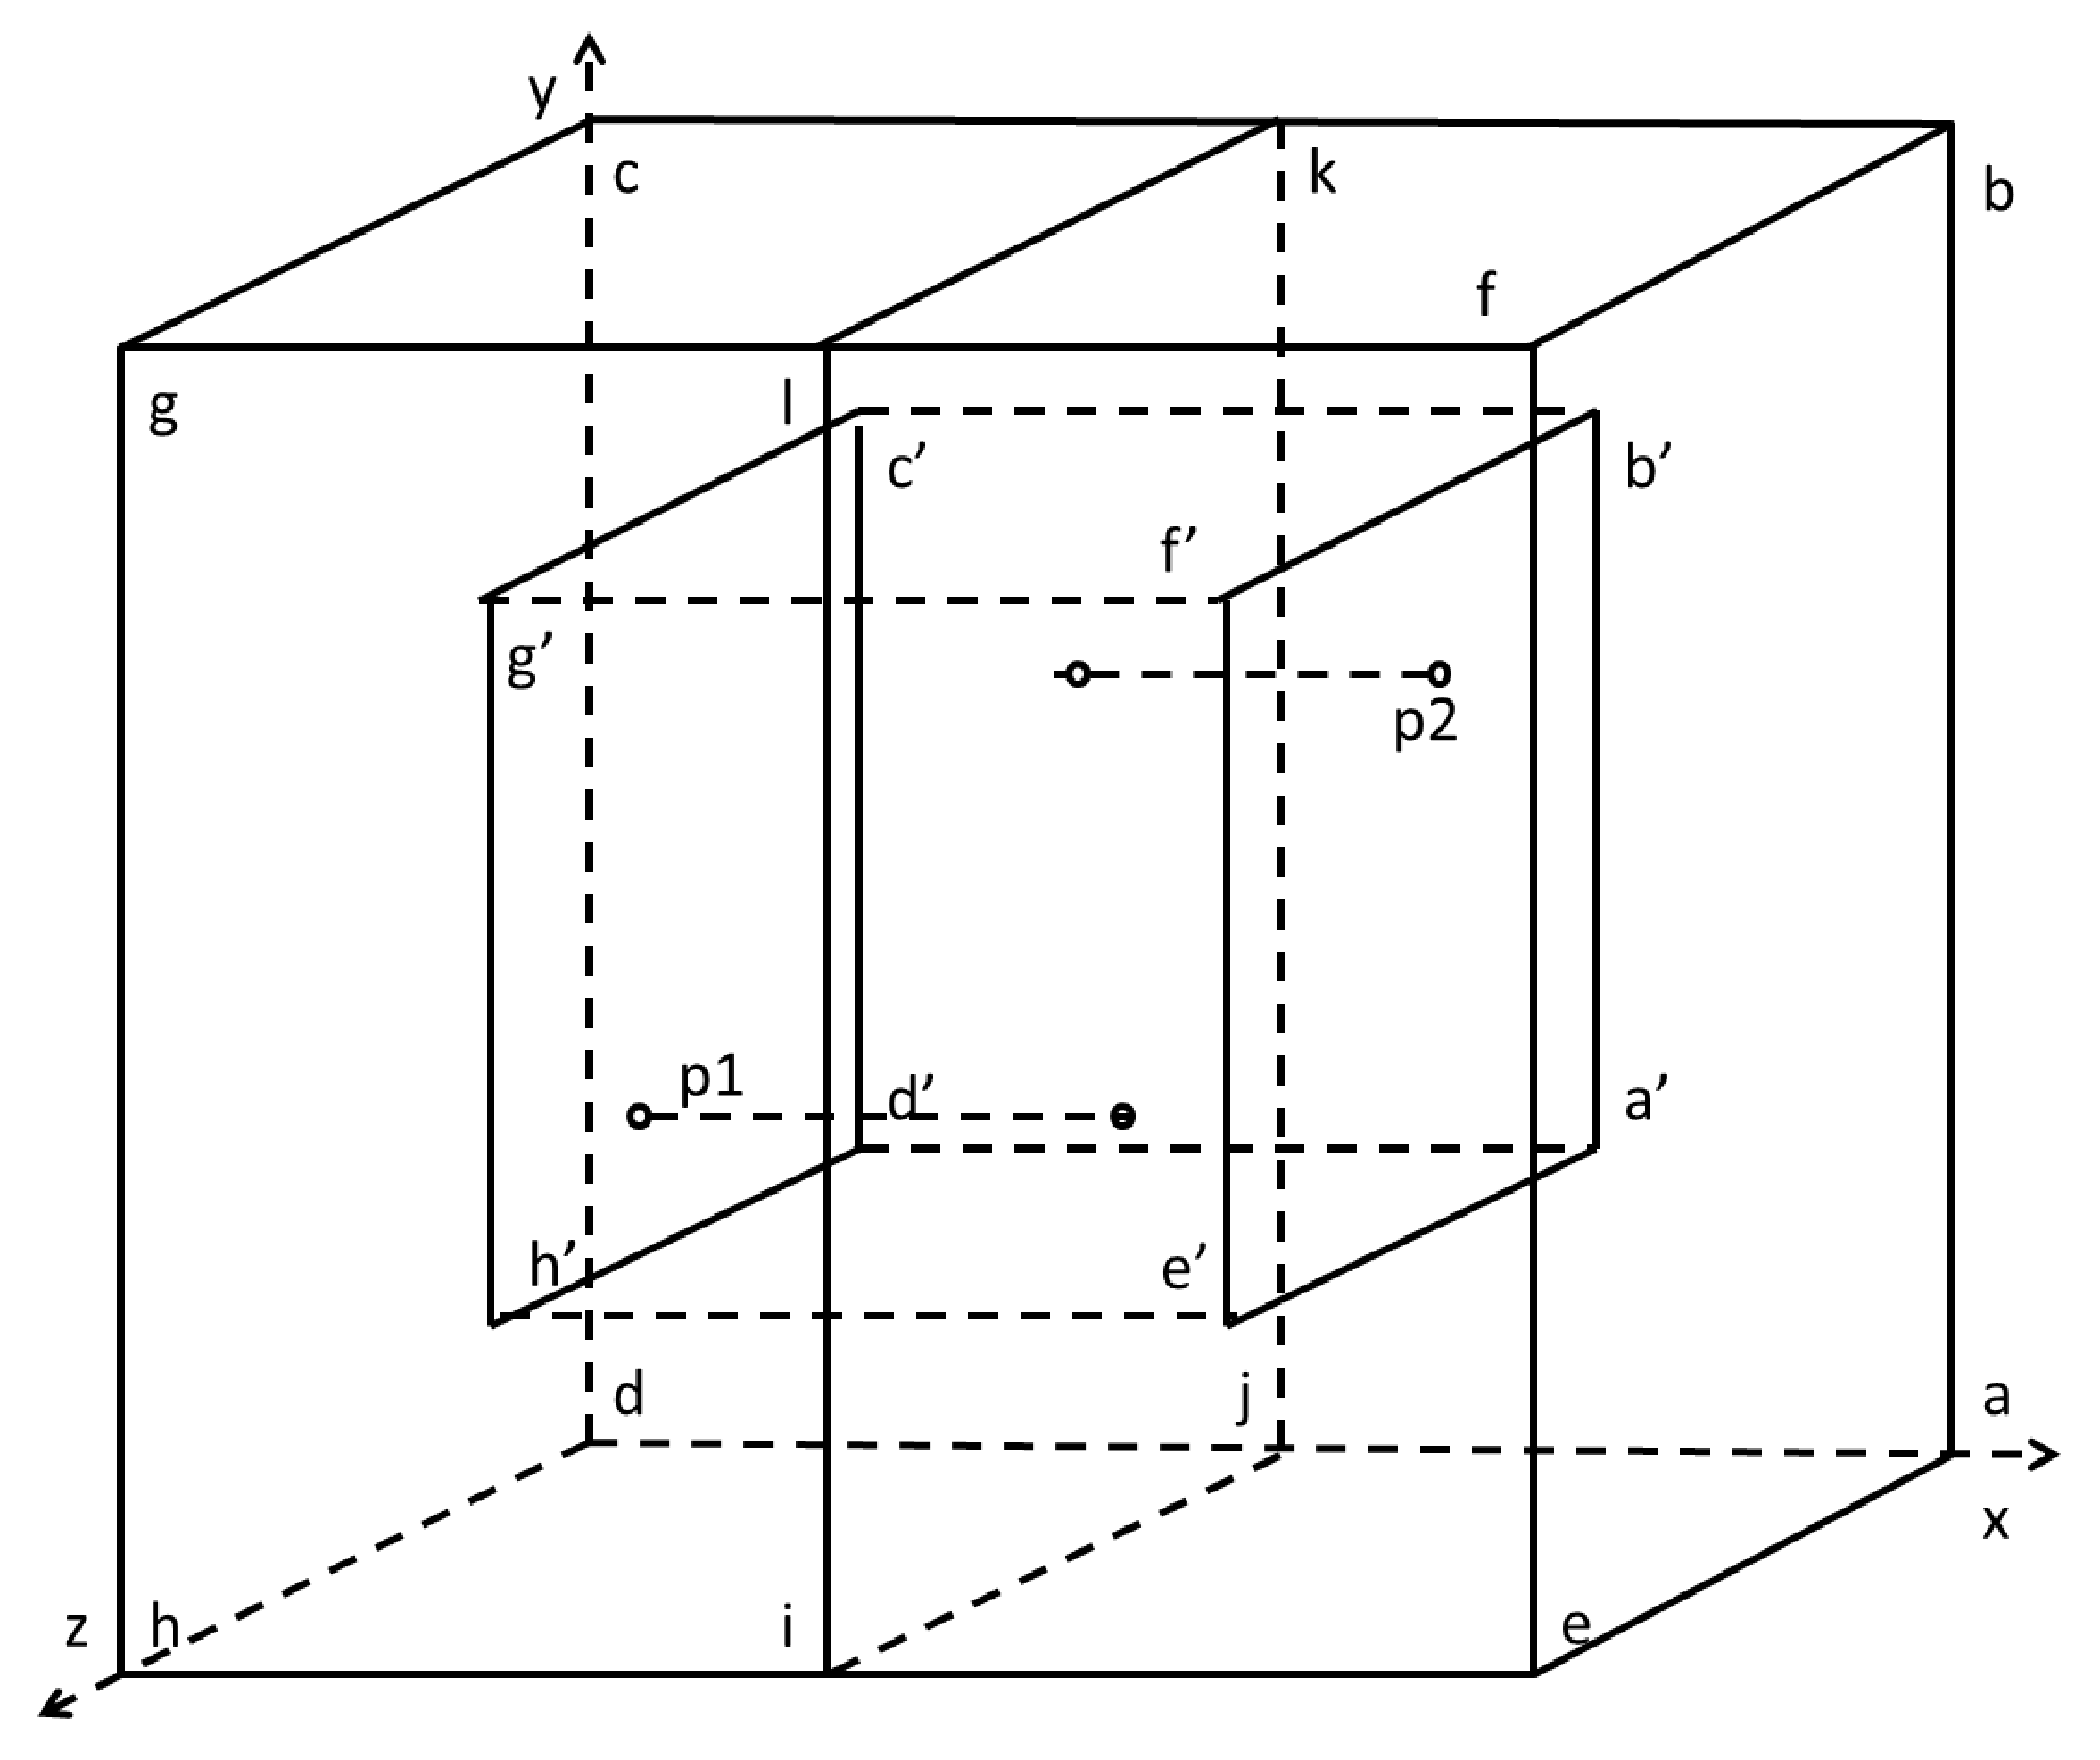
\includegraphics[width=2.5in]{figures/init_3D.eps}
\label{fig:threed}
\end{figure}

The $3$-D initial algorithm for orthogonal range query is pretty
straightforward and diagramed in \figref{threed}. Instead of center line,
we now have a center plane. In \figref{threed}, assuming $\id{x}$ is the
longest dimension and the first to reduce, we have a center face $\Box
\id{ijkl}$ to partition the entire grid into two parts. All the points
on the left-hand/right-hand side will reduce from center plane to itself
and store it as $\id{prefix/suffix\_grid}$. All the query range spanning
across the center plane can now be answered by two $2$-D queries. Then
recurse on both left and right parts of the center plane will cover all
$3$-D query ranges.

The meta-algorithm for $3$-D is also similar to the case of $2$-D, we
just need to reduce on all three dimensions to bring the preprocessing
complexity from $O(n_1 n_2 n_3 f(n_1) f(n_2) f(n_3))$ down to $O(n_1
n_2 n_3 f^*(n_1) f^*(n_2) f^*(n_3))$. The exact procedure is omitted
here.

\subsecput{init-2D}{Pseudo-code for the $2$-D initial algorithm}

\begin{figure}[!ht]
\small
\begin{codebox}
\Procname{$\proc{Init-2D}(\id{grid}, \id{x_0}, \id{x_1}, \id{y_0}, \id{y_1}; \proc{input\_1D\_algo}, \proc{op})$}
\li     $prefix\_grid \gets$ \New $((\id{x_1} - \id{x_0}) * (\id{y_1} - \id{y_0})$
\li     $suffix\_grid \gets$ \New $((\id{x_1} - \id{x_0}) * (\id{y_1} - \id{y_0})$
\li     \Comment Assuming we apply divide-and-conquer on dimension \id{x}
\li     \If $\id{x_1} - \id{x_0} <= 1$
\li         \Then \Return \Comment if the size of longer dimension $ <= 1$ then return
\li         \Else 
\li              $mid\_point \gets (\id{x_0} + \id{x_1})/2$
\li              \Comment Copy the starting point of prefix (on the right side of $mid\_point$)
\li              \Comment and suffix (on the left side of $mid\_point$)
\li              \For $y \gets \id{y_0}$ \To $\id{y_1}$
\li                  \Do $\id{suffix\_grid}[mid\_point-1][y] \gets \id{grid}[mid\_pont-1][y]$
\li                      $\id{prefix\_grid}[mid\_point][y] \gets \id{grid}[mid\_point][y]$ \End
\li              \Comment Reduce on all suffix
\li              \For $x \gets mid\_point-2$ \Downto $x_0$ 
\li                  \Do \For $y \gets \id{y_0}$ \To $\id{y_1}$
\li                      \Do $\id{suffix\_grid}[x][y] \gets \proc{op}(\id{grid}[x][y], \id{suffix\_grid}[x+1][y])$ \End \End
\li              \Comment Reduce on all prefix
\li              \For $x \gets mid\_point+1$ \To $x_1$
\li                  \Do \For $y \gets \id{y_0}$ \To $\id{y_1}$
\li                      \Do $\id{prefix\_grid}[x][y] \gets \proc{op}(\id{prefix\_grid}[x-1][y], \id{grid}[x][y])$ \End \End
\li              \Comment Apply the input $1$D algorithm on reduced prefix/suffix grid
\li              \Parfor $x \gets \id{x_0}$ \To $\id{x_1}$
\li                  \Do $\proc{input\_1D\_algo}(\id{suffix\_grid}[x][], \id{y_0}, \id{y_1}, \id{op})$
\li                      $\proc{input\_1D\_algo}(\id{prefix\_grid}[x][], \id{y_0}, \id{y_1}, \id{op})$ \End
\li              \Comment Recursively call \id{Init-2D} algorithm on the left side
\li              \Spawn $\proc{Init-2D}(\id{grid}, \id{x_0}, \id{mid\_point-1}, \id{y_0}, \id{y_1}; \id{input\_1D\_algo}, \id{op})$ 
\li              \Comment Recursively call \proc{Init-2D} algorithm on the right side
\li                     $\proc{Init-2D}(\id{grid}, \id{mid\_point}, \id{x_1}, \id{y_0}, \id{y_1}; \id{input\_1D\_algo}, \id{op})$ 
\li              \Sync \End
\end{codebox}
\caption{Initial $2$-D algorithm}
\label{fig:init-2D-algo}
\end{figure}

\subsecput{apdx-meta-2D}{Pseudo-code for the $2$-D meta algorithm}

% May put pseudo-code into appendix??
\begin{figure}[!ht]
\small
\begin{codebox}
\Procname{$\proc{Meta-2D}(\id{grid}, \id{x_0}, \id{x_1}, \id{y_0}, \id{y_1}; \id{REC}, \proc{input\_2D\_algo}, \proc{input\_1D\_algo}, \proc{op})$}
\li     \Comment Asssuming we do the data reduction on dimension $\id{x}$
\li     $seg\_size \gets \log(\id{x_1} - \id{x_0})$
\li     \Comment Depending on $\id{REC}$ level, we partition the seg\_size into $\log (\id{x_1} - \id{x_0})$, or $\log^* (\id{x_1} - \id{x_0})$, $\log^{**} (\id{x_1} - \id{x_0})$, $\ldots$
\li     \For $i \gets 0$ \To $REC$ 
\li         \Do $seg\_size \gets * seg\_size$ \End
\li     $n\_segs \gets (\id{x_1} - \id{x_0})/seg\_size$
\li     $promoted\_grid \gets $ \New $(n\_segs * (\id{y_1} - \id{y_0}))$
\li     $prefix\_grid \gets $ \New $((\id{x_1} - \id{x_0}) * (\id{y_1} - \id{y_0}))$
\li     $suffix\_grid \gets $ \New $((\id{x_1} - \id{x_0}) * (\id{y_1} - \id{y_0}))$
\li     \For $i \gets 0$ \To $n\_segs$
\li         \Do \For $j \gets 0$ \To $\id{y_1} - \id{y_0}$
\li             \Do \Comment $\proc{Reduce}$ apply input partial sum operator $\proc{op}$ over range $[i*seg_size, (i+1)*seg_size][j]$ 
\zi                 \Comment and return the reduced result into $promoted\_grid[i][j]$
\li                 $promoted\_grid[i][j] \gets \proc{Reduce}(i, j, \proc{op})$ 
\li                 \Comment $\proc{Reduce\_prefix}$ apply input partial sum operator $\proc{op}$ over range $[i*seg\_size, (i+1)*seg\_size][j]$ 
\zi                 \Comment and reduce the data relative to the beginning point of the segment ($i*seg_size$)
\li                 $prefix\_grid[i][j] \gets \proc{Reduce\_prefix}(i, j, \proc{op})$
\li                 \Comment $\proc{Reduce\_suffix}$ apply input partial sum operator $\proc{op}$ over range $[i*seg\_size, (i+1)*seg\_size][j]$ 
\zi                 \Comment and reduce the data relative to the end point of the segment ($(i+1)*seg_size$)
\li                 $suffix\_grid[i][j] \gets \proc{Reduce\_suffix}(i, j, \proc{op})$ \End \End
\li     \Comment Apply \proc{input\_2D\_algo} on the $promoted\_grid$
\li     $\proc{input\_2D\_algo}(promoted_grid, 0, n_segs, \id{y_0}, \id{y_1}; \id{REC-1}, \proc{input\_1D\_algo}, \proc{op})$
\li     \Parfor $i \gets 0$ \To $n\_segs$
\li         \Do \Comment Apply \proc{Meta-2D} itself onto the segments of $[i * seg\_size, (i+1) * seg\_size, \id{y_0}, \id{y_1}]$
\li             $\proc{Meta-2D}(\id{grid}, i * seg\_size, (i+1) * seg\_size, \id{y_0}, \id{y_1}; \id{REC}, \proc{input\_2D\_algo}, \proc{input\_1D\_algo}, \proc{op})$ \End
\li     \Parfor $i \gets \id{x_0}$ \To $\id{x_1}$
\li         \Do \Comment Apply the input $1$D algorithm on reduced prefix/suffix grid
\li             $\proc{input\_1D\_algo}(prefix\_grid[i], \id{y_0}, \id{y_1}, \proc{op})$
\li             $\proc{input\_1D\_algo}(suffix\_grid[i], \id{y_0}, \id{y_1}, \proc{op})$ \End
\end{codebox}
\caption{Meta $2$-D algorithm}
\label{fig:meta-2D-algo}
\end{figure}

\subsecput{apdx-meta-non-orthogonal}{Supplemental material for meta-algorithm for non-orthogonal range queries}

\begin{figure*}[t!]
\centering
\includegraphics[width=3in]{figures/meta_right_triangle.eps}
\vspace{-2cm}
\label{fig:meta-right-triangle}
\caption{Meta-algorithm for right triangular query in $2$-D grid.}
\end{figure*}

\subsecput{apdx-expr}{Experimental results of static partial sum problem}
\begin{figure*}[!ht]
\centering
\subfigure[Preprocessing time of meta-algorithm for $1$-D grid.]{\includegraphics[clip,width=3in]{figures/meta_1D_PP.eps}
\label{fig:meta-1D-PP}}
\hfill
%\hspace{0.01cm}
\subfigure[Preprocessing time of meta-algorithm for $2$-D grid]{\includegraphics[clip,width=3in]{figures/meta_2D_PP.eps}
\label{fig:meta-2D-PP}
}
\caption{Performance data of meta-algorithm's Preprocessing time for $1$-D and $2$-D grid}
\label{fig:meta-PP}
\end{figure*}

\begin{figure*}[!ht]
\centering
\subfigure[Query time of meta-algorithm for $1$-D grid]{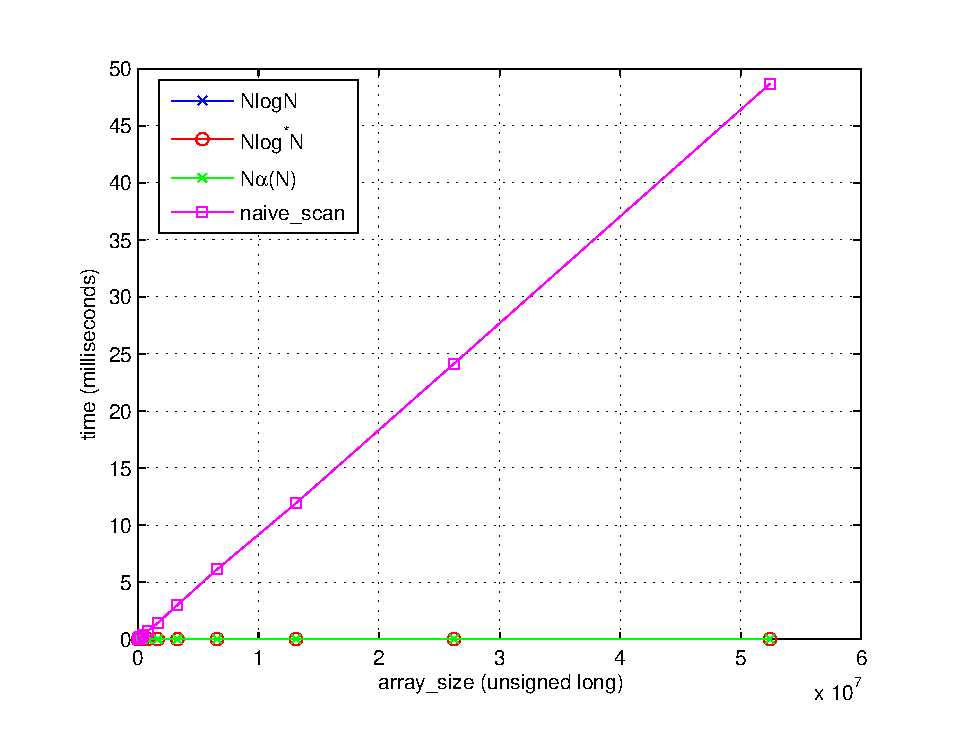
\includegraphics[clip,width=3in]{figures/meta_1D_query.eps}
\label{fig:meta-1D-query}}
\hfill
%\hspace{0.01cm}
\subfigure[Query time of meta-algorithm for $2$-D grid]{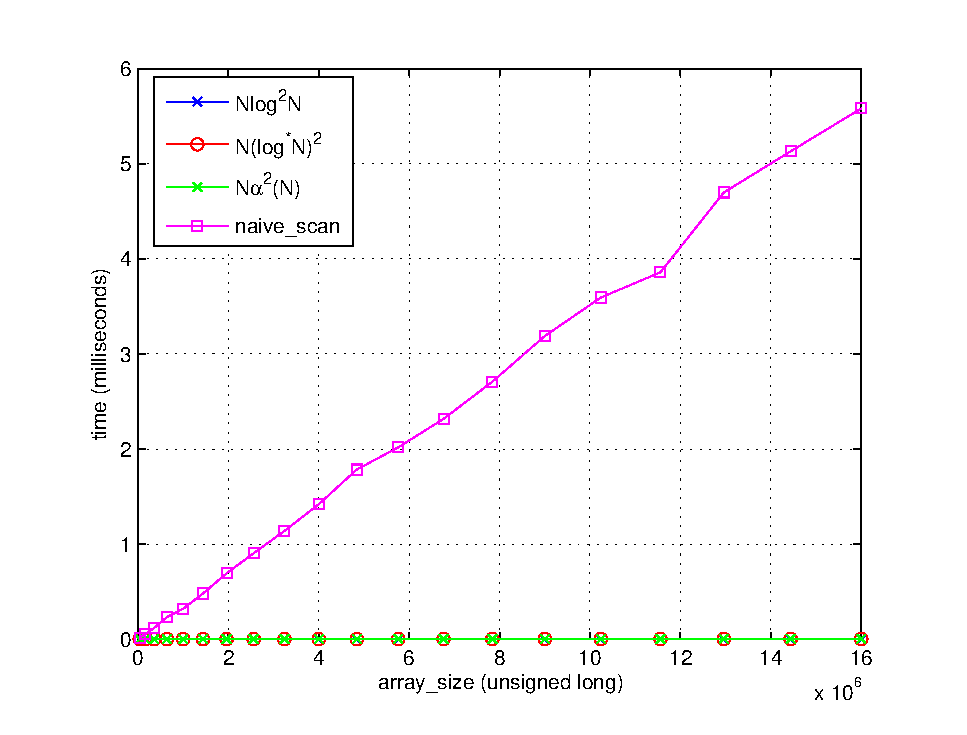
\includegraphics[clip,width=3in]{figures/meta_2D_query.eps}
\label{fig:meta-2D-query}
}
\caption{Performance data of meta-algorithm's Query time for $1$-D and $2$-D grid}
\label{fig:meta-query}
\end{figure*}


